\section{Versuchsaufbau}

Das Interferometer wurde auf einem schwingungsgedämpften optischen Tisch aufgebaut, als Lichtquelle wurde ein HeNe-Laser mit Wellenlänge $\lambda=633 nm$ verwendet. Der Lichtstrahl wurde durch einen Teleskopaufbau, bestehend aus einer Zerstreuungslinse mit Brennweite $f=-30.0 mm$ und einer Sammellinse mit Brennweite $f=200.0 mm$, die im Abstand von 17 cm zueinander aufgestellt wurden, aufgeweitet. Durch den Teleskopaufbau wird der Strahl zunächst aufgeweitet und dann wieder zu einem Parallelstrahl zusammengeführt. Dies ist notwendig, da eine zu starke Aufweitung bzw. Divergenz des Strahls eine Messung oder Zählung unmöglich machen würde, da der Kontrast des Interferenzbildes dadurch zu gering wäre. Nach dem Teleskopaufbau wurde der Strahl zunächst über zwei Spiegel parallel zur Tischebene ausgerichtet und dann in den halbdurchlässigen Spiegel geleitet. Der transmittierte Anteil des Strahls traf auf einen fest montierten Spiegel, der reflektierte Anteil traf auf einen auf einer Schiene beweglich montierten Spiegel. Hinter dem beweglichen Spiegel wurde der Edelstahlstab (Werkstoffnummer 1.4301), dessen Länge zu $l=28.9\pm0.1 cm$ gemessen wurde, eingespannt. In den Stab wurde ein kleines Loch gebohrt, sodass ein Temperaturfühler die Kerntemperatur des Stabes messen konnte. Der Temperaturfühler wurde an ein Sensor-CASSY 2 angeschlossen und die Messwerte über CASSYLab ausgelesen. Das entstehende Interferenzmuster wurde schließlich noch durch eine Zerstreuungslinse mit Brennweite $f=-100.0 mm$ aufgeweitet, um es besser sichtbar zu machen und auf eine Wand abgebildet.

\begin{figure}
\centering
	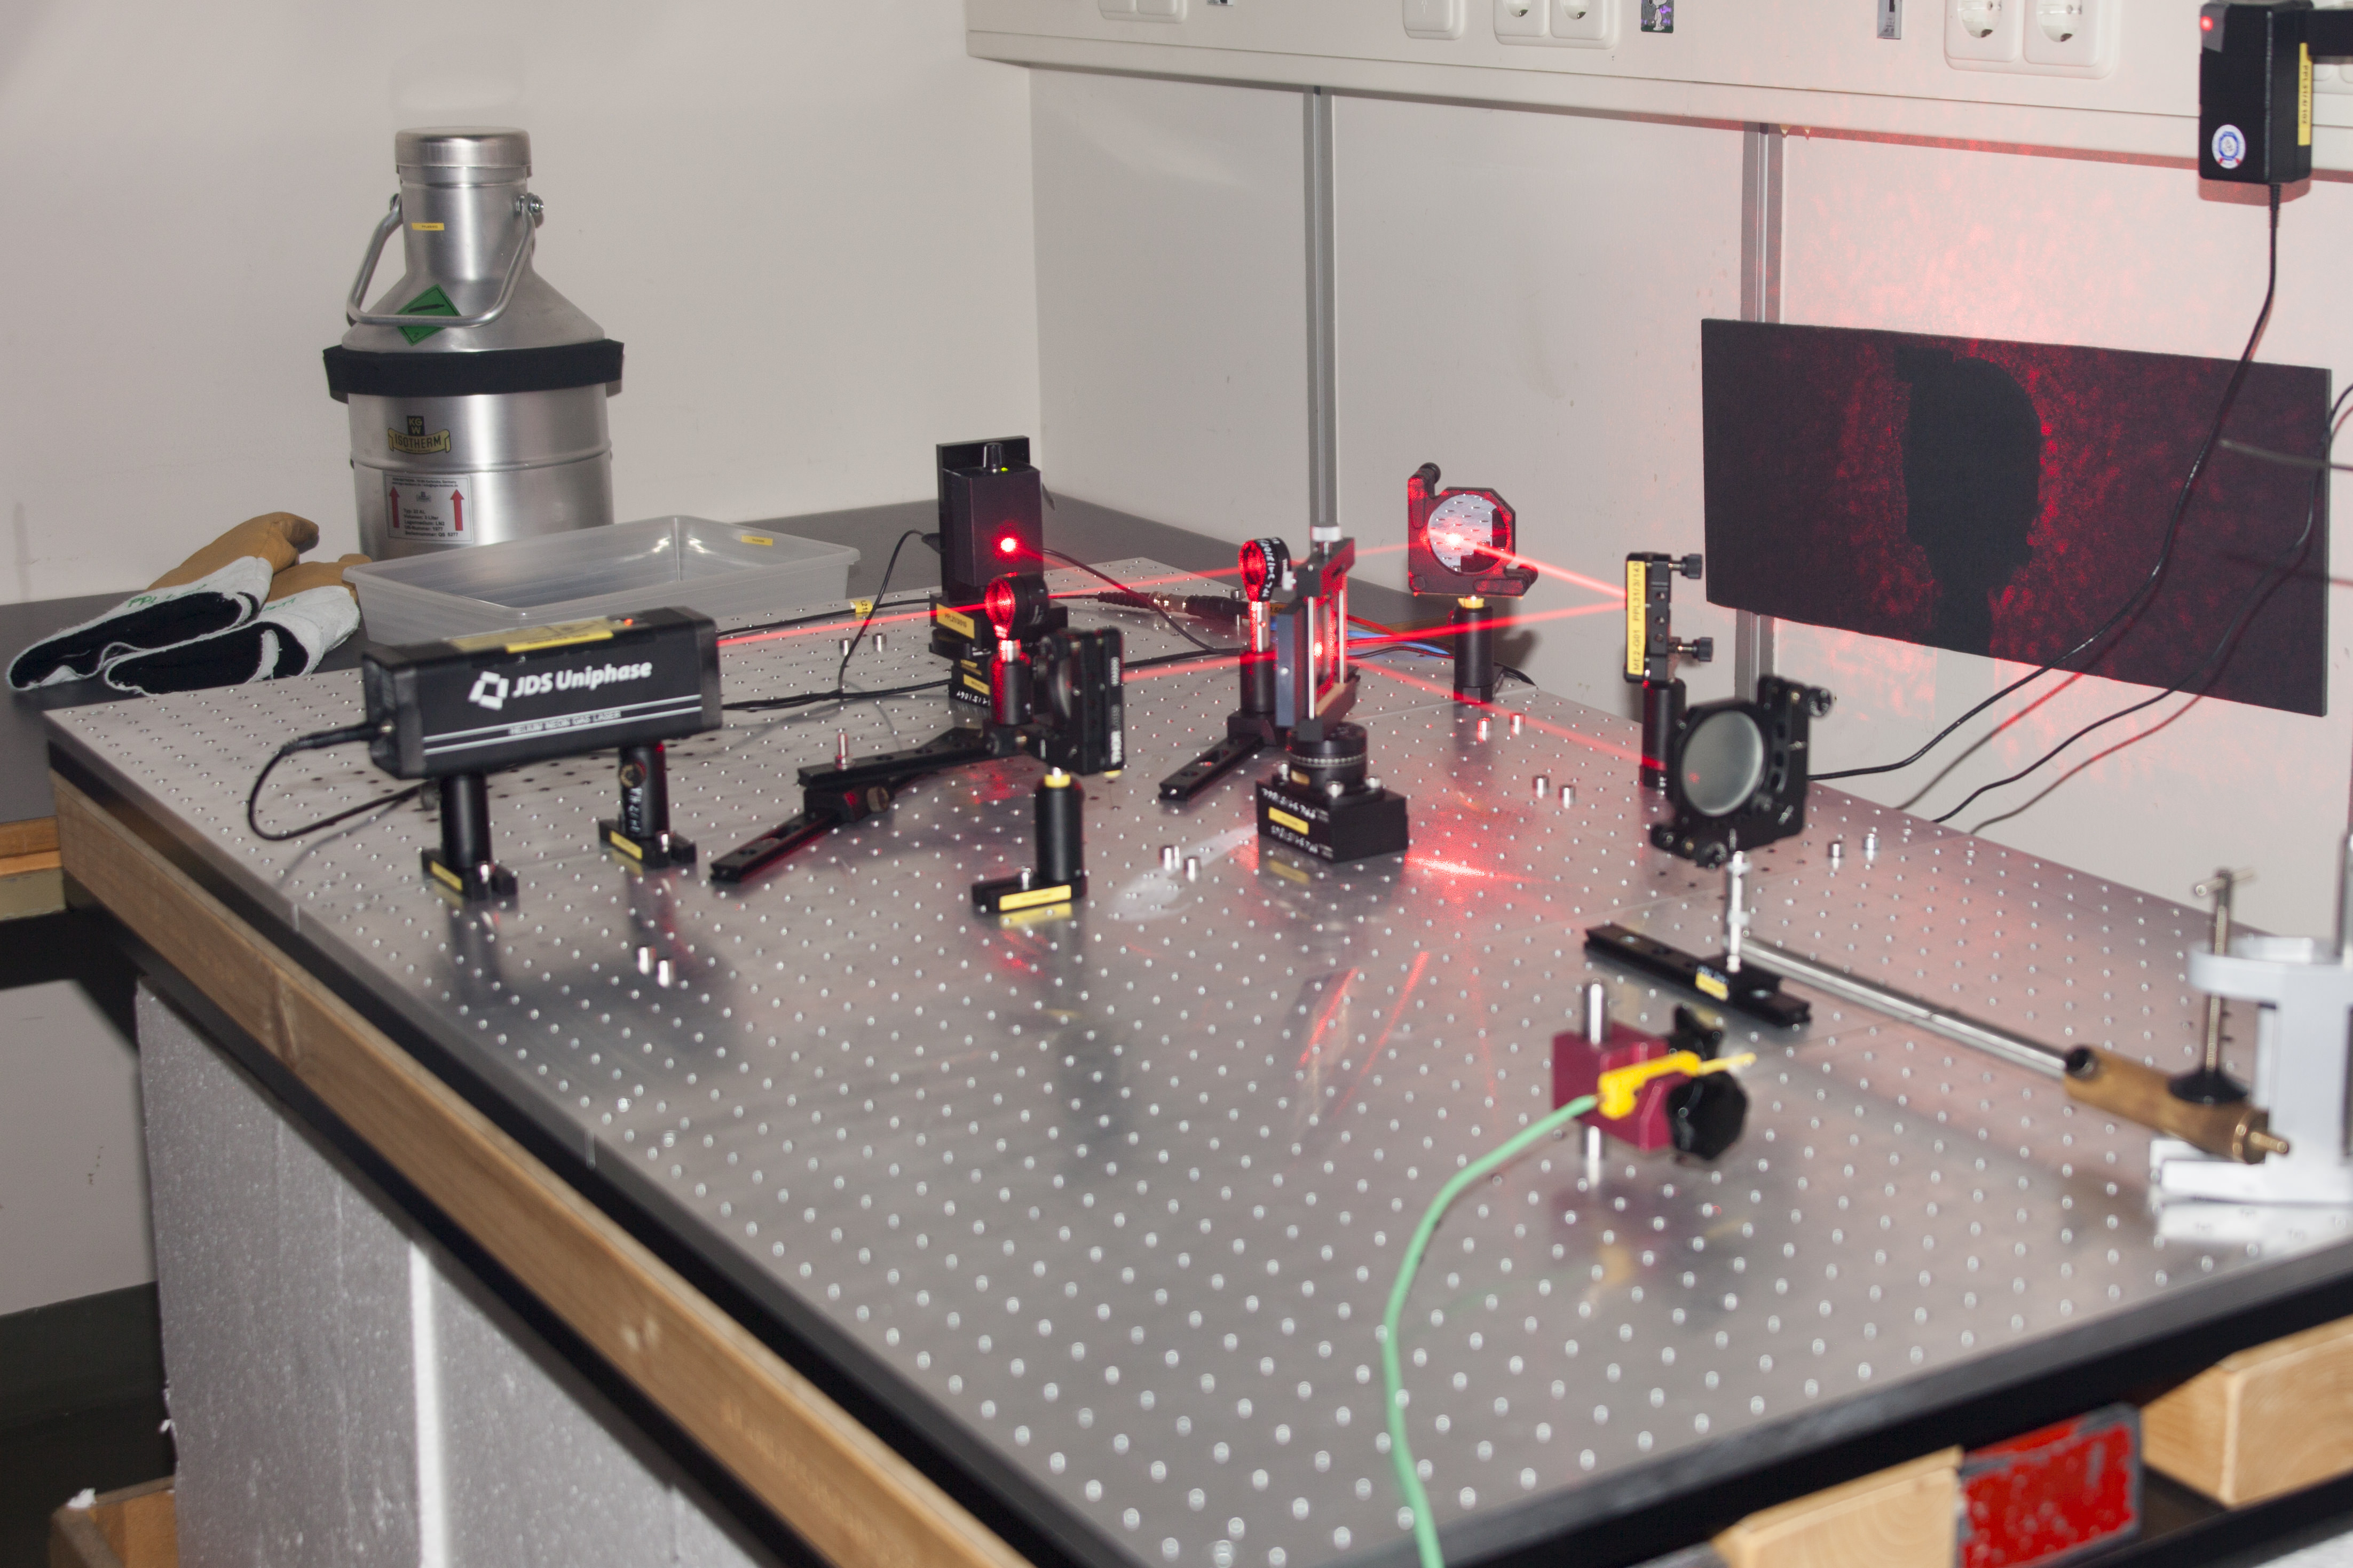
\includegraphics[width=.8\textwidth]{images/versuchsaufbau.jpg}
	\caption{Fotografie des Versuchsaufbaus nach Zeichnung in Abb. \ref{pic:skizze_versuchsaufbau}}
\end{figure}

\begin{landscape}
\begin{figure}
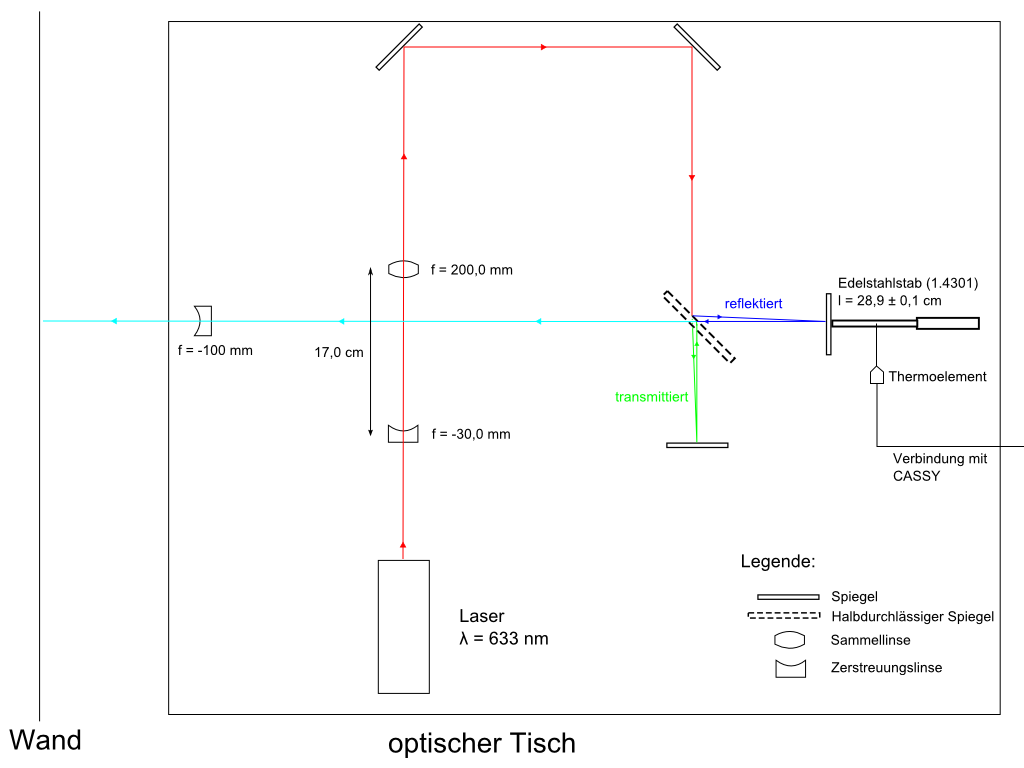
\includegraphics[height=\textwidth]{images/bitmap.png}
\caption{Skizze des Versuchsaufbaus, nicht maßstabsgetreu} 
\label{pic:skizze_versuchsaufbau}
\end{figure}
\end{landscape}

\section{Versuchsdurchführung}
\subsection{Messung}
Der Edelstahlstab wurde in ein Bad aus flüssigem Stickstoff ($T=-180^{\circ}C$) eingetaucht, aufgrund des Leidenfrost-Effekts war jedoch eine Abkühlung bis zu dieser Temperatur nicht möglich. Die Messung wurde bei einer gemessenen Temperatur von $T=-130^{\circ}C$ begonnen. Diese Art der Temperaturänderung des Stabs wurde gewählt, da die Ausdehnung des Stabs durch Aufheizung aus der Umgebungsluft gleichmäßiger ist als beispielsweise durch Aufheizen des Stabs mittels Heizdraht o.Ä..

Die Messung bestand daraus, die an einem Referenzpunkt an der Wand \enquote{vorbeilaufenden} Maxima zu zählen. Die Zählung aller Maxima wäre stark fehleranfällig gewesen, also wurden die Maxima in 10-Sekunden-Intervallen gezählt, d.h. die Anzahl der Maxima, die innerhalb von 10 Sekunden am Referenzpunkt vorbeiliefen.  Dann wurde 10 Sekunden pausiert, danach wurde die nächste zehnsekündige Messung gestartet. 

\subsection{Probleme}
Die Durchführung des Versuchs gestaltete sich insgesamt schwierig. Das Interferenzmuster war trotz schwingungsgedämpftem Aufbau anfällig gegen Erschütterungen. Auch eine sehr genaue Justierung des Interferometers war notwendig, da schon kleinste Verkippungen der Spiegel zusätzliche Streifenmuster erzeugten, die sich mit dem eigentlichen, d.h. durch den Strahlteiler erzeugten, Interferenzmuster überlagerten.

Ursprünglich war eine elektronische Messung mit CASSY geplant, bei der das Interferenzmuster auf den Sensor einer Fotodiode abgebildet werden sollte, sodass aus den Spannungsmaxima und -minima die Interferenzmaxima und -minima erkennbar sein sollten.
In der Praxis war dies jedoch sehr schwierig, da die Ausschläge aufgrund der geringen Intensität des Lichts nach Aufweitung und Durchgang durch den Strahlteiler so gering waren, dass sie selbst bei maximaler Verstärkung an der Diode nicht vom Grundrauschen der Diode unterscheidbar waren. Dies konnte zwar durch geringere Aufweitung (Teleskopaufbau) teilweise behoben werden (d.h. auf einem Oszilloskop waren die Maxima und Minima deutlich zu erkennen), bei einer probeweise durchgeführten Messung mit CASSY waren die Daten jedoch nicht verwertbar, auch bei einer zweiten Messung mit höherer zeitlicher Auflösung waren keine klaren Ausschläge zu erkennen, sodass die Messung schließlich doch per Hand durchgeführt wurde.
